\documentclass[11pt]{article}
\usepackage{ctex} %中文
\usepackage[utf8]{inputenc}
\usepackage[a4paper, left=3cm, right=3cm, top=2.5cm, bottom=2.5cm]{geometry} 

\usepackage{graphicx}
\usepackage{subcaption}
\usepackage{float}
\usepackage{amsmath, amsthm, amssymb}

\usepackage{booktabs}
\usepackage{fancyhdr}  % 导入宏包
\setlength{\headheight}{14pt}
\pagestyle{fancy}      % 启用 fancyhdr 页面样式

\fancyhf{}             % 清空原有的页眉和页脚设置
\fancyhead[L]{Chapter 06 }
\fancyhead[C]{}
\fancyhead[R]{Computer Network}

\fancyfoot[C]{\thepage}

\renewcommand{\headrulewidth}{0.4pt} % 设置页眉线粗细
\renewcommand{\footrulewidth}{0.4pt}

%代码块格式
\usepackage{listings}
\usepackage{xcolor} %设置颜色
%\usepackage{setspace} % 用于调整行间距

%\usepackage{parskip}  

% 定义代码样式：
\lstset{
    language=Python,
    basicstyle=\ttfamily\small,
    %numbers=left,
    numberstyle=\tiny\color{gray},
    stepnumber=1,
    breaklines=true,
    frame=shadowbox,
    commentstyle=\color{green!60!black},
    keywordstyle=\color{blue},
    stringstyle=\color{purple},
    backgroundcolor=\color{white},
    showstringspaces=false,
    showspaces=false
}


\title{\textbf{Homework of Chapter 06 \\ \small Computer Network}}
\author{姓名：唐凯峰 \qquad 学号：524030910124}
\date{\today}

\begin{document}
\maketitle 
\section*{简答题}
\subsection*{1. } 
已知数据D = 1010101010，生成多项式G = 10011. 由于G有5位，所以余数R有4位。 
由CRC原理：$D \cdot 2^r $ XOR $R = nG$，
用$D \cdot 2^r$除以G，即可得到余数R。

用$D \cdot 2^r = 10101010100000$除以$G = 10011$，做模2异或除法，计算得到余数：
\[R = 0100\]

\subsection*{2. }
会发生冲突。因为两个节点同时发送，并且传播时延$t_{drop}$小于分组发送时间$L/R$，
导致一个节点的信号在信道上传播到另一个节点后，另一个节点仍然在发送自己的分组。这导致两个信号会在信道上发生重叠，发生碰撞。

\subsection*{3. }
ARP 查询是广播帧，这是因为发送ARP请求时主机还不知道目的MAC地址，无法单播，只能使用广播地址。这样局域网内所有设备都会收到这个请求；只有IP地址匹配的设备会ARP回复。

ARP响应是单播帧：这是因为目标主机解封ARP查询报文后知道了发送方的MAC地址，因此ARP响应可以直接封装在目的MAC地址的报文中，以单播帧的形式发送给请求方。

\subsection*{4. }
假设六个节点A-F连接到一个独立端口，分别设为1-6，即($A \to 1$), ($B \to 2$), \dots。交换表初始化为空。
下表是每一次事件后的交换表条目更新。 

\begin{table}[H] % h:当前位置, t:页顶, b:页底, p:新页
  \centering % 表格居中
  \begin{tabular}{cc}
    \toprule % 顶部粗线
    事件 & 交换表条目 \\
    \midrule % 中部细线
    初态 & None \\
    事件(i) & <$B \to 2$> \\
    事件(ii) & <$B \to 2$, $E \to 5$>  \\
    事件(iii) & <$B \to 2$, $E \to 5$,$A \to 1$> \\
    事件(iv) & <$B \to 2$, $E \to 5$, $A \to 1$> \\
    \bottomrule % 底部粗线
  \end{tabular}
\end{table}

交换机收到帧后，会先学习源地址；然后查看目的地址。如果不知道目的地址则需要泛洪；如果已知则单播发送。
通过不断自学习来更新转发表条目。基于这个原理，可以得到： 
\begin{itemize}
    \item (i) 帧将被泛洪，发送到除B以外的所有链路上。
    \item (ii) 帧将单播转发到B链路上。
    \item (iii) 帧将单播转发到B链路上。
    \item (iv) 帧将单播转发到A链路上 。
\end{itemize}

\section*{Wireshark实验: Ethernet and ARP}
实验环境：Ubuntu24.04虚拟机。

\subsection*{Part I. 捕获和分析以太网帧}
根据要求完成浏览\textit{US Bill of Rights}的抓包实验，捕获的HTTP GET消息如图1所示。

\begin{figure}[H] 
    \centering % 使图片居中
    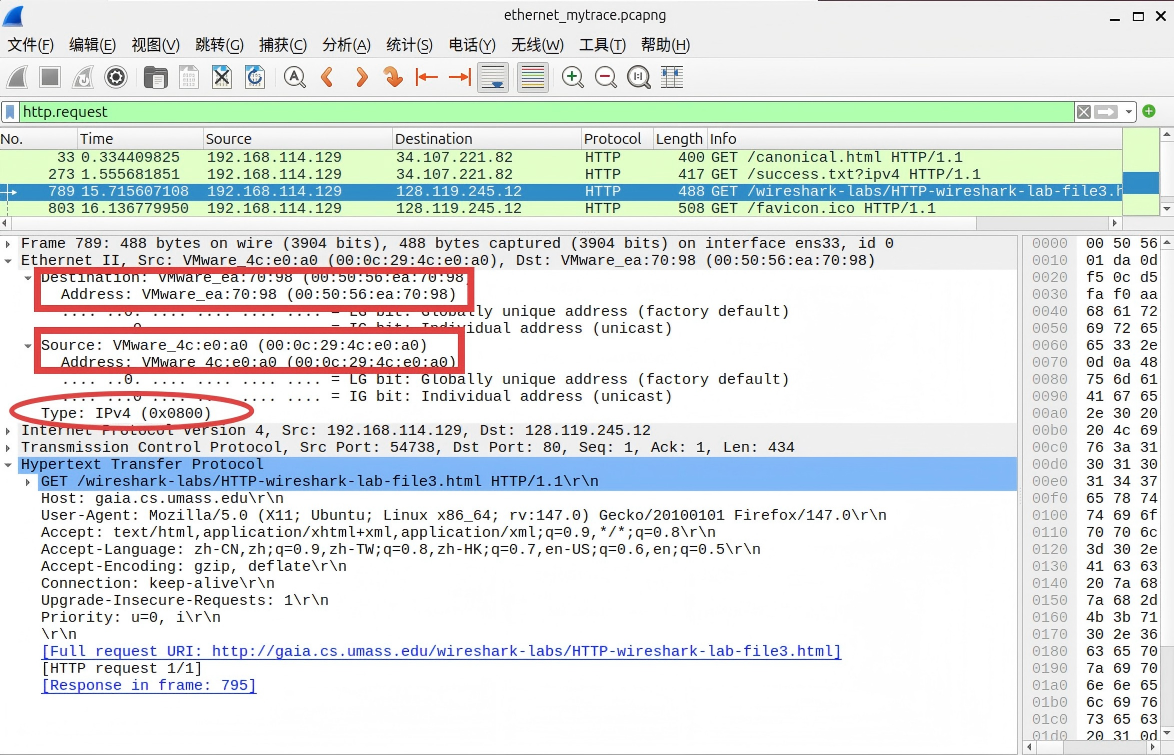
\includegraphics[width=0.85\textwidth]{./figures/1.png} 
    \caption{\fangsong Wireshark捕获的HTTP GET消息} % 设置标题
\end{figure}

\newpage 

由观察Wireshark抓包并分析，可以回答以下问题： 

\textbf{1. 我的计算机的48位以太网MAC地址：}由Ethernet II部分中Source的显示，可以看到本机的 48 位以太网地址是：
00:0c:29:4c:e0:a0。

\textbf{2. 以太网帧中的48位目的地址：}由Ethernet II部分中Destination的显示，可以看出48位目的地址：
00:50:56:ea:70:98。这不是\texttt{gaia.cs.umass.edu}的MAC地址！

原因：以太网帧只能在本地链路中传输。本机访问远程服务器时，会先把帧发送给默认网关。显示的应该是默认网关(第一跳路由器)的MAC。

\textbf{3. 承载 HTTP GET 请求的以太网帧中，两字节 Type 字段的十六进制值是多少？对应哪个上层协议？}

观察图1中的重点批注：Ethernet II的Type部分，可以看到IPv4 (0x0800)，说明
两字节 Type 字段为：0x0800，对应的上层协议是：IPv4。

\textbf{4. 从以太网帧的最开始算起，“GET” 中的 ASCII 字符 “G” 出现在第几个字节？}
继续观察图2展示的 Wireshark HTTP GET帧展示的详细内容，可以查看IP头部长度以及TCP头部长度：
\[\text{IP Header Length } = 20 \text{ bytes}\]
\[\text{TCP Header Length } = 20 \text{ bytes}\]

从图3的以太网帧头部信息中结合右侧的十六进制偏移量，可以看到Ethernet 头部长度占据14 bytes: 
\begin{itemize}
    \item Destination MAC: 6 bytes; 
    \item Source MAC: 6 bytes; 
    \item Type: 2 bytes. 
\end{itemize}

\begin{figure}[H] 
    \centering % 使图片居中
    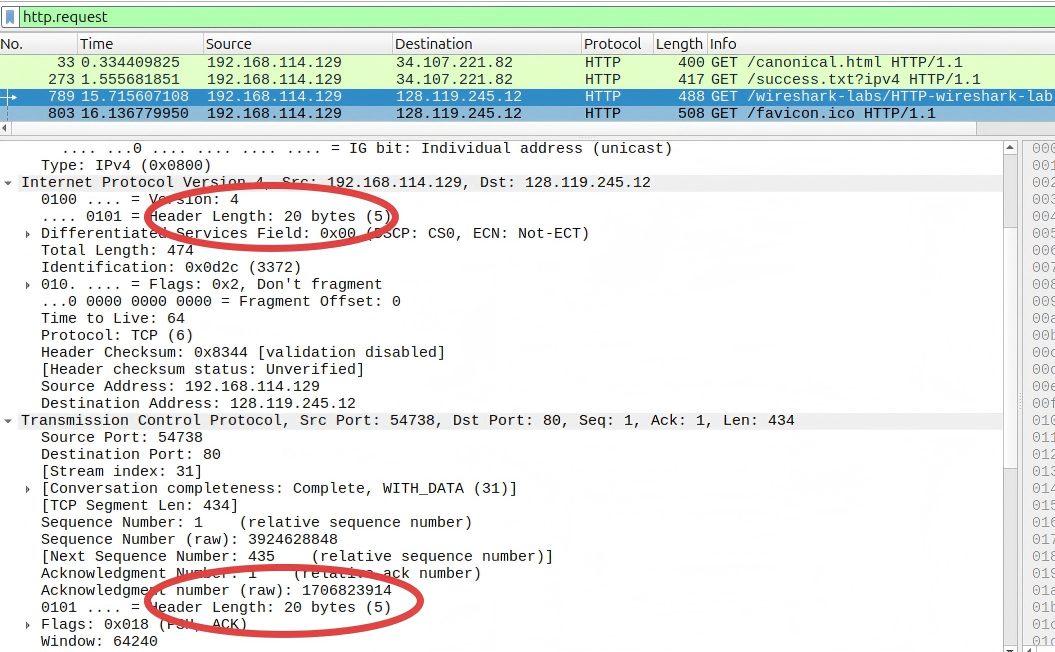
\includegraphics[width=0.85\textwidth]{./figures/2.png} 
    \caption{\fangsong HTTP GET帧捕获的IP和TCP信息} % 设置标题
\end{figure}

\begin{figure}[H] 
    \centering % 使图片居中
    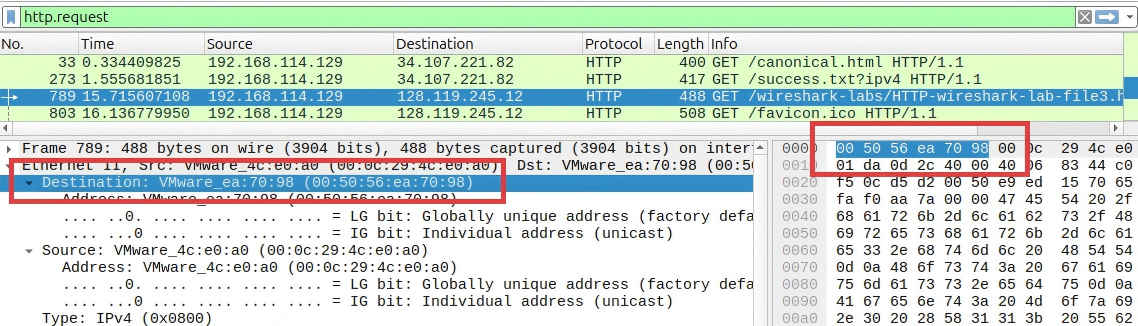
\includegraphics[width=0.85\textwidth]{./figures/3.png} 
    \caption{\fangsong HTTP GET帧捕获的以太网头部信息} % 设置标题
\end{figure}

因此 HTTP 数据即将开始开始的位置为：14 + 20 + 20 = 54 (bytes) 位置。
所以“GET” 中的 G 出现在第 55 个字节。

接下来，分析包含HTTP Response消息的以太网帧内容，如图4所示。

\begin{figure}[H] 
    \centering % 使图片居中
    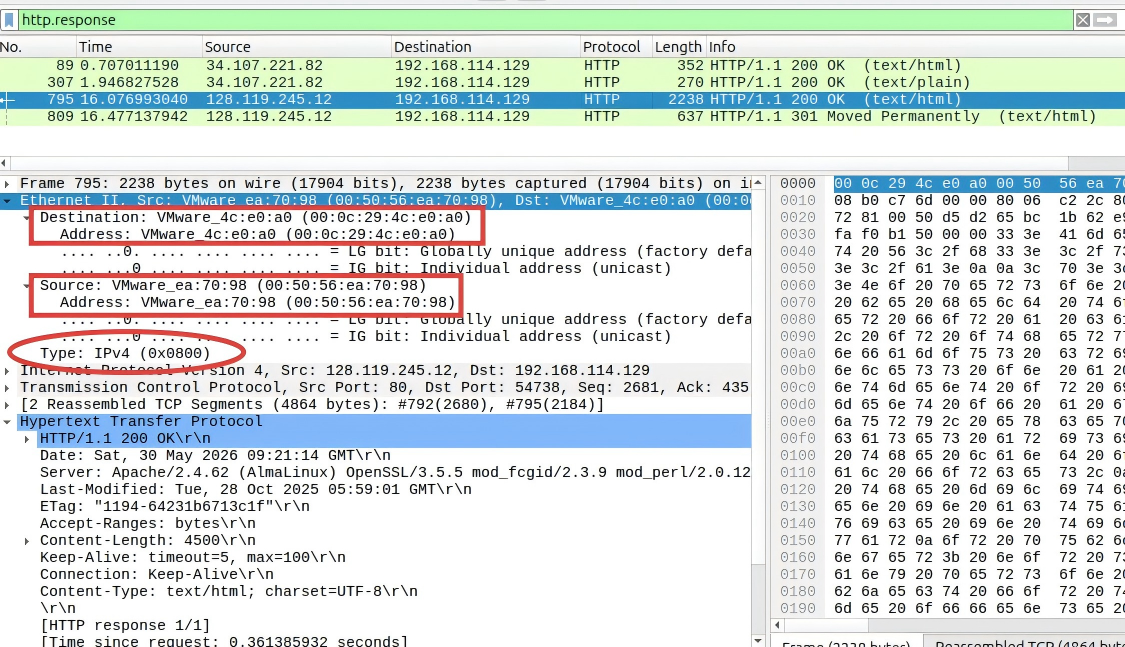
\includegraphics[width=0.85\textwidth]{./figures/response.png} 
    \caption{\fangsong Wireshark捕获的HTTP Response以太网帧的信息} % 设置标题
\end{figure}

根据观察以及分析，可以回答下列问题：

\textbf{5. 以太网源地址：}00:50:56:ea:70:98。这不是本机的MAC地址，也不是
gaia.cs.umass.edu的 MAC 地址。由题目2可知，本地的默认网关才具有这个地址。

原因是远程服务器返回的 IP 数据报到达本地网络后，会由默认网关重新封装成以太网帧再发送给本机。
因此，在最后一跳链路中，以太网帧的源 MAC 是默认网关的 MAC。

\textbf{6. 以太网帧中的目的地址：}00:0c:29:4c:e0:a0。
这是我的Linux虚拟机网卡ens33的MAC地址。

\textbf{7. 给出两字节 Type 字段的十六进制值。这对应于哪个上层协议？}

与HTTP GET帧相同，HTTP 响应帧的 Ethernet II Type 字段为：0x0800。它对应的上层协议是：IPv4。

\textbf{8. 从以太网帧的最开始算起，“OK” 中的 ASCII 字符 “O” 出现在第几个字节？}

此题的计算思路与第4题相同：经过观察验证，同样按 Ethernet 14 字节、IP 20 字节、TCP 20 字节计算。

需要注意的是，HTTP 响应状态行是“HTTP/1.1 200 OK”，从 HTTP 数据部分开始数，O的位置应该为13。
因此O字母的偏移量是：14+20+20+13=67。应该是出现在第 68个字节。

\textbf{9. 携带了构成完整 HTTP “200 OK ...” 响应消息数据的以太网帧数量：}通过使用过滤器：
\begin{lstlisting}
tcp.stream eq 31 && ip.src == 128.119.245.12 && tcp.len > 0
\end{lstlisting}

结果显示如图5所示，服务器返回给本机的TCP数据帧共有两个。

\begin{figure}[H] 
    \centering % 使图片居中
    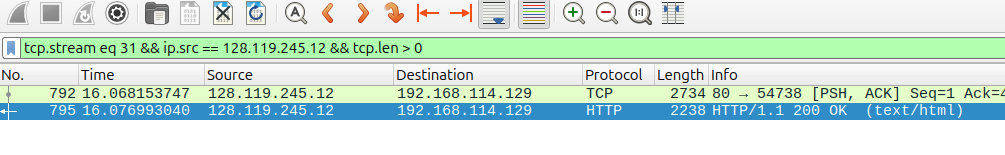
\includegraphics[width=0.8\textwidth]{./figures/4.png} 
    \caption{\fangsong 携带200 OK消息的以太网帧} % 设置标题
\end{figure}

\qquad 

\subsection*{Part II. ARP 协议}
首先通过命令\texttt{arp -a}查看计算机上ARP缓存的内容。据此回答两个问题：

\textbf{10. ARP 缓存中存储的条目数量：}2条。其中
192.168.114.2 是默认网关；
192.168.114.254 是同一虚拟网络中的另一个 VMware 相关网络设备。

\begin{figure}[H] 
    \centering % 使图片居中
    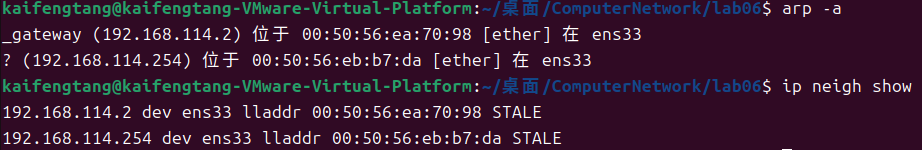
\includegraphics[width=0.8\textwidth]{./figures/arp_a.png} 
    \caption{\fangsong 命令行执行的\texttt{arp -a}输出} % 设置标题
\end{figure}

\textbf{11. ARP 缓存中显示的每个条目包含的内容：}IP 地址、
对应的 MAC 地址、
地址类型，例如 ether、
所属网络接口，例如 ens33、
主机名或设备名，如果系统能够解析出来，例如 \_gateway。

\qquad 

接下来，清除ARP缓存，开启抓包并浏览网页，通过过滤器“arp”获取ARP查询和回复消息，
如图7和图8所示。
观察并分析信息，回答下列问题：

\textbf{12. 包含计算机发送的 ARP 请求消息的以太网帧中，源地址的十六进制值是多少？}

ARP 请求帧的源 MAC 地址为：00:0c:29:4c:e0:a0，这就是虚拟机网卡 ens33 的 MAC 地址。

\textbf{13. 包含计算机发送的 ARP 请求消息的以太网帧中，目的地址的十六进制值是多少？}

Destination 显示的是以太网广播地址 ff:ff:ff:ff:ff:ff。
它不对应某一台具体设备，而表示局域网内所有设备都会接收该帧。这是因为发送方此时不知道目标对应的 MAC 地址。

\begin{figure}[H] 
    \centering % 使图片居中
    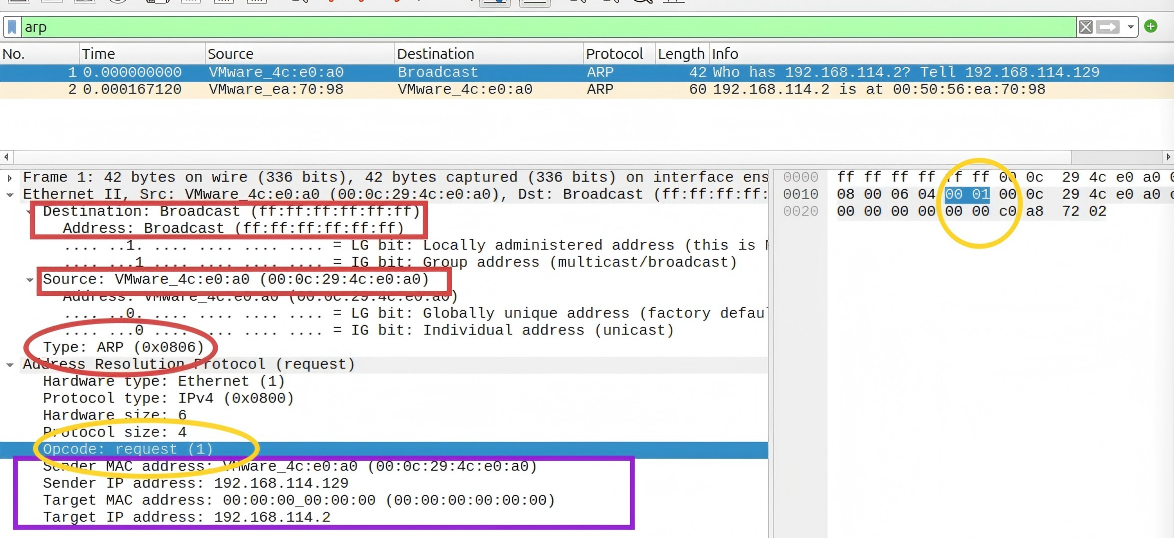
\includegraphics[width=0.8\textwidth]{./figures/arp1.png} 
    \caption{\fangsong Wireshark 捕获的ARP查询消息} % 设置标题
\end{figure}

\begin{figure}[H] 
    \centering % 使图片居中
    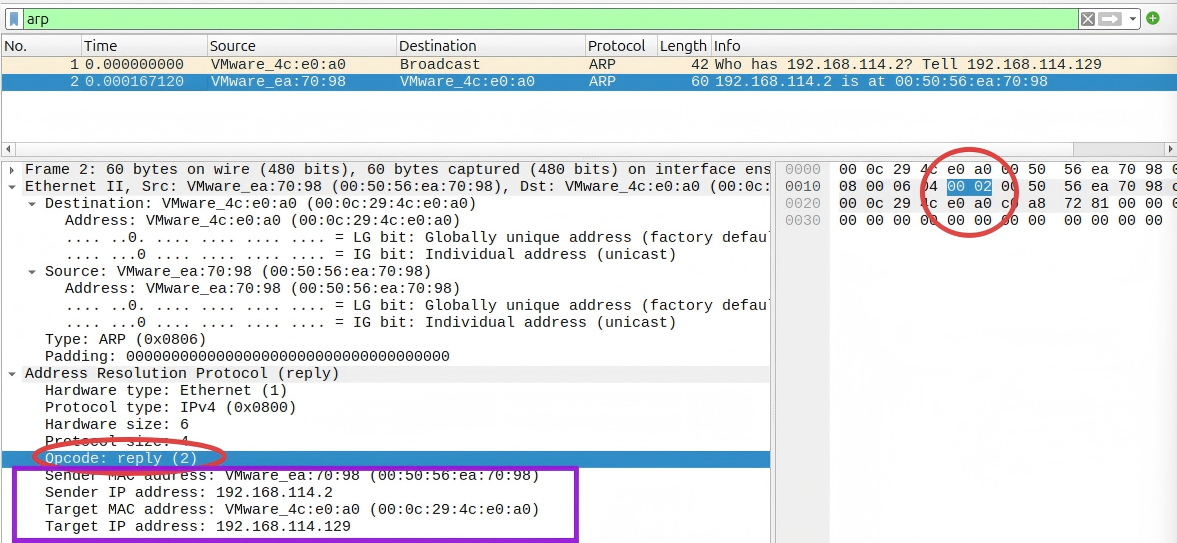
\includegraphics[width=0.8\textwidth]{./figures/arp2.png} 
    \caption{\fangsong Wireshark 捕获的ARP回复消息} % 设置标题
\end{figure}

\textbf{14. 两字节的以太网帧 Type 字段的十六进制值：}0x0806，对应的上层协议是ARP。

\textbf{15. 从以太网帧的最开始算起，ARP 操作码 opcode 字段从第几个字节开始？}

与之前的分析相同，以太网头部长度共14字节；观察图7中的ARP报文，可以看到opcode 前面有：
\[\text{Hardware type: 2 bytes}\]
\[\text{Protocol type: 2 bytes}\]
\[\text{Hardware size: 1 byte}\]
\[\text{Protocol size: 1 byte}\]

总共为6 bytes。因此 opcode 距离以太网帧开头的偏移量为：
14 + 6 = 20。$\implies$ARP opcode 字段从第 21 个字节开始。

\textbf{16. opcode 字段的值：} 由图7中批注出来的Opcode: request (1)，
以及圈出来的右侧对应的十六进制表示，可以得到opcode的字段值为0x0001。

\textbf{17. ARP 请求消息是否包含发送方的 IP 地址？}

包含。从ARP报文信息中的Sender IP address就可以看出，IP地址为192.168.114.129。这就是我的虚拟机本机IP地址。

\textbf{18.  ARP 请求消息中，正在请求对应以太网 MAC 地址的设备 IP 地址是什么？}

由Target IP address 可以看出正在请求其 MAC 地址的设备 IP 是：192.168.114.2，这就是本机的默认网关IP地址。 

\textbf{19. 接收到的 ARP 回复消息中，opcode 字段的值：}Opcode: reply (2)，对应0x0002。

\textbf{20. 与计算机发出的 ARP 请求中指定的 IP 地址相对应的以太网 MAC 地址：}ARP Reply 第 2 号帧显示：
192.168.114.2 is at 00:50:56:ea:70:98，因此，IP 地址 192.168.114.2 对应的 MAC 地址是：
00:50:56:ea:70:98。

这也与 HTTP GET 帧中的目的 MAC 地址一致，说明本机访问远程服务器时，首先把以太网帧发送给默认网关。

\textbf{21. 为什么在跟踪文件中，没有看到针对这些其他 ARP 请求消息发送的 ARP 回复？}

因为 ARP 请求是广播帧，目的 MAC 地址为：ff:ff:ff:ff:ff:ff。
所以同一局域网中的所有主机都能看到这些 ARP Request。

但是 ARP Reply 是单播帧，只有回复方会把 ARP Reply 发送给发起请求的主机。

\qquad 

\textbf{附加问题：}

\textbf{\textit{EX-1. }如果使用 arp -s 手动添加了错误的 MAC 地址，会发生什么？}

如果 IP 地址是正确的，但 MAC 地址填错了，那么本机向该 IP 地址发送数据时，会把以太网帧发往错误的 MAC 地址。

这可能导致：目标主机收不到数据、数据帧被错误发送给其他设备。
如果错误 MAC 地址属于攻击者，攻击者可能截获或转发流量，形成攻击。

\textbf{\textit{EX-2. }动态 ARP 条目默认保留多长时间？}
从图6中的\texttt{ip neigh show}命令执行情况来看，
STALE 表示该 ARP 条目已经过了可达状态时间，但尚未被系统删除。如果之后需要再次通信，系统可能会重新确认该邻居项。

通过查阅资料，Linux可以通过以下命令查看动态邻居项的基础可达时间：

\begin{figure}[H] 
    \centering % 使图片居中
    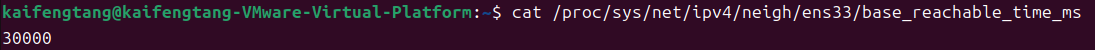
\includegraphics[width=0.9\textwidth]{./figures/ex2.png} 
\end{figure}


执行该命令，最终返回值为30000，也就是30秒。这说明
动态 ARP 条目的 REACHABLE 可达状态默认约为 30 秒；随后会进入 STALE 状态，但不会立即删除。

\end{document}
